\documentclass[a4paper, 12pt, svgnames]{article}

\usepackage{preambule}

\title{Variabilités intrinsèques des SNe Ia et leurs conséquences sur les
paramètres cosmologiques}

\fancyhead[L]{\scriptsize \textsc{Variabilités intrinsèques des SNe Ia}}

\begin{document}

\thispagestyle{empty}
\noindent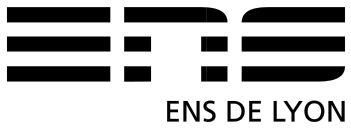
\includegraphics[height=2cm]{General_figures/logoens.png} \hfill

\includegraphics[height=2cm]{General_figures/logoucbl.png} \hfill

\includegraphics[height=2cm]{General_figures/logounivlyon.png}\vfill

\noindent\begin{tabularx}{\linewidth+27pt}{@{} l X r @{} }
{\textsc{Master Science de la matière}} & & Année 2018--2019\hspace*{1cm}\\
{\textit{École Normale Supérieure de Lyon}} & & \textsc{Nicolas} Nora\hspace*{1cm}\\
{\textit{Université Claude Bernard Lyon I}} & & M2 Physique\hspace*{1cm}
\end{tabularx}

\begin{center}\vfill\hrule\vspace*{8pt}

\textbf{\huge Variabilités intrinsèques des SNe Ia et leurs conséquences sur les
paramètres cosmologiques}\\

\hrule\vfill

\parbox{15cm}{\small\textbf{Résumé}:
In order to achieve a 1\% determination of the Dark Energy state parameter w,
both statistic and systematic uncertainties need to be dealt with. If getting
more data can reduce the statistic ones, only the study of the physical behavior
of our astral objects of study, namely the supernovae of type Ia (SNe Ia for
short) can impact the systematic ones. In this report, we'll discuss how
establishing the evolution of SNe Ia's stretch parameter as a function of the
redshift can be of use for this goal.}\vspace{0.5cm}

\parbox{15cm}{\small\textbf{Mots-clés}:
Cosmologie, supernovae}\vspace{0.5cm}

\parbox{15cm}{Stage supervisé par:\\
\textbf{\textsc{RIGAULT} Mickaël}, Chercheur\\
\href{mailto:rigault@ipnl.in2p3.fr}{rigault@ipnl.in2p3.fr}\\
\href{https://www.ipnl.in2p3.fr/perso/rigault/}{Site personnel}\bigbreak
Institut de Physique des Deux Infinis\\
{\textit{Université Lyon 1\\4 rue Enrico Fermi -- bâtiment Dirac\\
69622 Villeurbanne Cedex}}\\
\url{https://www.ipnl.in2p3.fr}}\vspace{.5cm}\vfill


\includegraphics[width=.3\textwidth]{General_figures/IP2I.png}
\end{center}\vfill \hfill \today
\newpage
\thispagestyle{empty}
\setcounter{page}{0}

\appsec{Remerciements}{sec:ack}

Je tiens à remercier toutes les personnes qui ont contribué, de près ou de loin,
à la réalisation de ce stage et de ce rapport de stage. En premier lieu, bien
évidemment, je remercie Mickaël \bsc{Rigault} pour son encadrement sans faille

\tableofcontents
\newpage

\section{Introduction}\label{sec:int}
\subsection{Le domaine de recherche}

La combinaison des observations et des prédictions théoriques du modèle du Big
Band indiquent que l'univers est en expansion. Lors de la découverte de cette
expansion, on pensait qu'elle devrait ralentir sous l'effet de la gravitation.
Cependant, l'utilisation des supernovae de type Ia (SNe Ia) par \bsc{Perlmutter
et al.}~\cite{perlmutter_measurements_1999}, \bsc{Riess et al.}
~\cite{riess_observational_1998} et \bsc{Schmidt et al.}
~\cite{schmidt_high-z_1998} a permis de mettre en évidence l'expansion
accélérée de l'Univers, découverte pour laquelle ils ont eu le prix Nobel de
physique de 2011. Il y aurait ainsi un phénomène allant à l'encontre des
effets gravitationnels, phénomène qui a été nommé « énergie noire » : la
cosmologie moderne vise entre aux à mieux comprendre la nature de cette énergie,
sa proportion dans l'Univers et les lois physiques auxquelles elle obéit.

\begin{itemize}
    \item Tension sur $H_0$? \bsc{Riess et al.} 2016 donne des valeurs en intro
\end{itemize}

\subsection{Diagramme de Hubble}
\begin{itemize}
    \item Mesure de magnitude, équations ;
    \item Dispersion naturelle, imprécision.
\end{itemize}
L'utilisation des SNe Ia se fait par la mesure de leur distance de luminosité.
La grandeur que les instrument mesure est en fait le flux de l'astre:
\[ F = \frac{L}{4\pi d²}\]
avec $L$ sa luminosité et $d$ la distance entre l'astre et le capteur.

\subsection{Les SNe Ia}
\begin{itemize}
    \item Spécificité astrophysique ;
    \item Pertinence cosmologique.
\end{itemize}

\subsection{Courbes de lumière}
\begin{itemize}
    \item Définitions ;
    \item Relations empiriques, équation corrigée.
\end{itemize}

\subsection{Incertitudes systématiques}
\begin{itemize}
    \item Importance dans les mesures actuelles ;
    \item Importance dans les mesures futures.
\end{itemize}

\subsection{Problème du progéniteur}
\begin{itemize}
    \item Progéniteur inconnus :
    \item L moyennes différentes avec $z$ ou échantillon ;
    \item Évolution du \textit{lsSFR}.
\end{itemize}

Parler du fait que le code est sur GitHub, et faire des références dans la
suite.

\section{Construction d'un échantillon complet}
\subsection{Effets de sélection}
\begin{itemize}
    \item Histogramme échantillons ;
    \item Rappel relation \textcolor{red}{brighter-slower} et conclusion.
\end{itemize}

\subsection{Méthode de détermination}
\begin{itemize}
    \item Modèle d'évolution ;
    \item Statistique poissonienne, itérations pour chaque échantillon.
\end{itemize}

\section{Modèle d'évolution}
\subsection{Origine du modèle}
\begin{itemize}
    \item Données \textcolor{orange}{SNF} ;
    \item Définition jeune/vieille d'après \bsc{Rigault et al.} 2018
\end{itemize}

\subsection{Implémentation aux échantillons}
\begin{itemize}
    \item Concordance avec \textcolor{orange}{SNF} seulement
    \item Modèle \textcolor{orange}{SNF} sur toutes les données
\end{itemize}

\subsection{Modifications et comparaisons}
\begin{itemize}
    \item Modification du modèle ;
    \item Implémentation d'autres modèles et résultats
\end{itemize}

\section{Conclusion}
Conclusion

\bibliographystyle{unsrt}
\bibliography{VIDSTIA}
\addcontentsline{toc}{section}{Bibliographie}

\end{document}
